% macro_usage_guide.tex
% Complete LaTeX Guide for Engineering Students

\documentclass[a4paper,11pt]{article}
\usepackage{school-macros}

\title{\LaTeX{} Gids voor Ingenieurs\\[0.5em]\large Van Basis tot Samenvatting}
\author{Engineering Study Guide}
\date{\today}

\begin{document}

\maketitle
\tableofcontents
\newpage

%=============================================================================
\section{Document Structuur}
%=============================================================================

Een basis \LaTeX{} document ziet er zo uit:
\begin{verbatim}
\documentclass[a4paper,11pt]{article}
\usepackage{school-macros}

\title{Titel}
\author{Auteur}
\date{\today}

\begin{document}
\maketitle
\tableofcontents

\section{Eerste Sectie}
Tekst hier...

\subsection{Subsectie}
Meer tekst...

\end{document}
\end{verbatim}

%=============================================================================
\section{Tekst Opmaak}
%=============================================================================

\subsection{Basis Stijlen}
\begin{tabular}{ll}
\verb|\textbf{vet}| & \textbf{vet} \\
\verb|\textit{cursief}| & \textit{cursief} \\
\verb|\underline{onderstreept}| & \underline{onderstreept} \\
\verb|\texttt{monospace}| & \texttt{monospace} \\
\verb|\emph{nadruk}| & \emph{nadruk} \\
\verb|\textsc{Small Caps}| & \textsc{Small Caps} \\
\end{tabular}

\subsection{Combineren}
\textbf{\textit{Vet én cursief}} met \verb|\textbf{\textit{tekst}}|

\subsection{Lettergroottes}
{\tiny tiny} {\scriptsize scriptsize} {\footnotesize footnotesize} {\small small} {\normalsize normal} {\large large} {\Large Large} {\LARGE LARGE} {\huge huge}

\subsection{Uitlijning}
\begin{verbatim}
\begin{center}
  Gecentreerde tekst
\end{center}



\begin{flushleft}
  Links uitgelijnd
\end{flushleft}

\begin{flushright}
  Rechts uitgelijnd
\end{flushright}
\end{verbatim}

\begin{center}
Dit is gecentreerde tekst
\end{center}

\subsection{Kleuren (met school-macros)}
\begin{itemize}
\item \verb|\concept{begrip}|: \concept{belangrijk concept} (blauw, vet)
\item \verb|\belangrijk{tekst}|: \belangrijk{waarschuwing} (rood, vet)
\item \verb|\keyterm{term}|: \keyterm{sleutelbegrip} (blauw accent)
\end{itemize}

%=============================================================================
\section{Wiskunde Modus — Basis}
%=============================================================================

\subsection{Inline vs Display}
\textbf{Inline} (in de tekst): De energie is $E = mc^2$ volgens Einstein.

\textbf{Display} (eigen regel):
\[ E = mc^2 \]

Of met nummering:
\begin{equation}
E = mc^2
\end{equation}

\subsection{Superscript en Subscript}
\begin{tabular}{ll}
\verb|$x^2$| & $x^2$ \\
\verb|$x^{10}$| & $x^{10}$ (meerdere tekens: accolades!) \\
\verb|$x_1$| & $x_1$ \\
\verb|$x_{12}$| & $x_{12}$ \\
\verb|$x_i^2$| & $x_i^2$ (beide tegelijk) \\
\verb|$a_{n+1}^{2k}$| & $a_{n+1}^{2k}$ \\
\end{tabular}

\subsection{Griekse Letters}
\begin{tabular}{llll}
\verb|\alpha| & $\alpha$ & \verb|\Alpha| & $A$ \\
\verb|\beta| & $\beta$ & \verb|\gamma| & $\gamma$ \\
\verb|\delta| & $\delta$ & \verb|\Delta| & $\Delta$ \\
\verb|\epsilon| & $\epsilon$ & \verb|\theta| & $\theta$ \\
\verb|\lambda| & $\lambda$ & \verb|\mu| & $\mu$ \\
\verb|\pi| & $\pi$ & \verb|\sigma| & $\sigma$ \\
\verb|\omega| & $\omega$ & \verb|\Omega| & $\Omega$ \\
\verb|\phi| & $\phi$ & \verb|\rho| & $\rho$ \\
\end{tabular}

\subsection{Veelgebruikte Symbolen}
\begin{tabular}{llllll}
\verb|\cdot| & $\cdot$ & \verb|\times| & $\times$ & \verb|\div| & $\div$ \\
\verb|\pm| & $\pm$ & \verb|\mp| & $\mp$ & \verb|\neq| & $\neq$ \\
\verb|\leq| & $\leq$ & \verb|\geq| & $\geq$ & \verb|\approx| & $\approx$ \\
\verb|\infty| & $\infty$ & \verb|\partial| & $\partial$ & \verb|\nabla| & $\nabla$ \\
\verb|\rightarrow| & $\rightarrow$ & \verb|\Rightarrow| & $\Rightarrow$ & \verb|\leftrightarrow| & $\leftrightarrow$ \\
\verb|\in| & $\in$ & \verb|\notin| & $\notin$ & \verb|\subset| & $\subset$ \\
\end{tabular}

%=============================================================================
\section{Wiskunde — Formules}
%=============================================================================

\subsection{Breuken}
\begin{tabular}{ll}
\verb|\frac{a}{b}| & $\frac{a}{b}$ \\
\verb|\frac{x^2 + 1}{2x}| & $\frac{x^2 + 1}{2x}$ \\
\verb|\dfrac{a}{b}| & $\dfrac{a}{b}$ (display-stijl in inline) \\
\end{tabular}

Snelle breuken (school-macros):
$\half$, $\third$, $\quarter$ met \verb|\half|, \verb|\third|, \verb|\quarter|

\subsection{Wortels}
\begin{tabular}{ll}
\verb|\sqrt{x}| & $\sqrt{x}$ \\
\verb|\sqrt{x^2 + y^2}| & $\sqrt{x^2 + y^2}$ \\
\verb|\sqrt[3]{x}| & $\sqrt[3]{x}$ (derdemachtswortel) \\
\verb|\sqrt[n]{x}| & $\sqrt[n]{x}$ (n-de machtswortel) \\
\end{tabular}

\subsection{Boxed — Belangrijke Formules}
\[ \boxed{F = ma} \]
\[ \boxed{E = \frac{1}{2}mv^2 + mgh} \]

\subsection{Sommaties en Integralen}
\[
\sum_{i=1}^{n} i = \frac{n(n+1)}{2} \qquad
\prod_{i=1}^{n} i = n!
\]

\[
\int_0^{\infty} e^{-x} \, dx = 1 \qquad
\iint_S f(x,y) \, dA \qquad
\oint_C \vec{F} \cdot d\vec{r}
\]

\subsection{Limieten}
\[
\lim_{x \to 0} \frac{\sin x}{x} = 1 \qquad
\lim_{n \to \infty} \left(1 + \frac{1}{n}\right)^n = e
\]

\subsection{Matrices}
\[
\begin{pmatrix} a & b \\ c & d \end{pmatrix} \quad
\begin{bmatrix} 1 & 0 \\ 0 & 1 \end{bmatrix} \quad
\begin{vmatrix} a & b \\ c & d \end{vmatrix} = ad - bc
\]

\subsection{Meerdere Vergelijkingen (align)}
\begin{align}
F &= ma \\
a &= \frac{dv}{dt} \\
v &= \frac{dx}{dt}
\end{align}

Zonder nummering met \verb|align*|:
\begin{align*}
P &= UI \\
  &= I^2 R \\
  &= \frac{U^2}{R}
\end{align*}

\subsection{Gevallen (cases)}
\[
|x| = \begin{cases}
x & \text{als } x \geq 0 \\
-x & \text{als } x < 0
\end{cases}
\]

%=============================================================================
\section{Lijsten}
%=============================================================================

\subsection{Opsomming (bullets)}
\begin{itemize}
\item Eerste punt
\item Tweede punt
  \begin{itemize}
  \item Sub-punt
  \end{itemize}
\end{itemize}

\subsection{Genummerd}
\begin{enumerate}
\item Stap één
\item Stap twee
\item Stap drie
\end{enumerate}

\subsection{Beschrijving}
\begin{description}
\item[Kracht] $F = ma$ — product van massa en versnelling
\item[Energie] $E = mc^2$ — massa-energie equivalentie
\item[Vermogen] $P = \frac{dE}{dt}$ — energie per tijdseenheid
\end{description}

%=============================================================================
\section{Tabellen}
%=============================================================================

\subsection{Basis Tabel}
\begin{center}
\begin{tabular}{|l|c|r|}
\hline
Links & Midden & Rechts \\
\hline
A & B & C \\
1 & 2 & 3 \\
\hline
\end{tabular}
\end{center}

\subsection{Professionele Tabel (booktabs)}
\begin{table}[H]
\centering
\caption{Materiaaleigenschappen}
\begin{tabular}{lcc}
\toprule
\textbf{Materiaal} & \textbf{$\rho$ [kg/m³]} & \textbf{$E$ [GPa]} \\
\midrule
Staal & 7850 & 210 \\
Aluminium & 2700 & 70 \\
Koper & 8960 & 120 \\
\bottomrule
\end{tabular}
\end{table}

\subsection{Brede Tabel (tabularx)}
\begin{table}[H]
\centering
\caption{Definities}
\begin{tabularx}{\linewidth}{l X}
\toprule
\textbf{Term} & \textbf{Definitie} \\
\midrule
Spanning & Kracht per oppervlakte-eenheid: $\sigma = F/A$ \\
\addlinespace
Rek & Relatieve verlenging: $\varepsilon = \Delta L / L_0$ \\
\bottomrule
\end{tabularx}
\end{table}

%=============================================================================
\section{Grafieken met TikZ/PGFPlots}
%=============================================================================

\subsection{Functie Plot}
\begin{center}
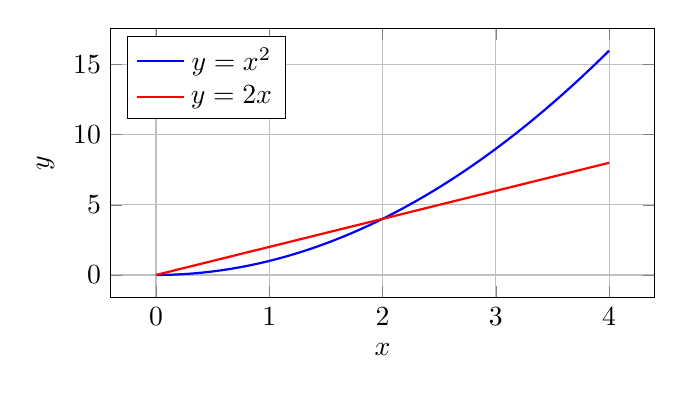
\begin{tikzpicture}
\begin{axis}[
    width=0.7\linewidth,
    height=5cm,
    xlabel={$x$},
    ylabel={$y$},
    grid=major,
    legend pos=north west
]
\addplot[blue, thick, domain=0:4, samples=50] {x^2};
\addlegendentry{$y = x^2$}
\addplot[red, thick, domain=0:4, samples=50] {2*x};
\addlegendentry{$y = 2x$}
\end{axis}
\end{tikzpicture}
\end{center}

\subsection{Data Plot met Punten}
\begin{center}
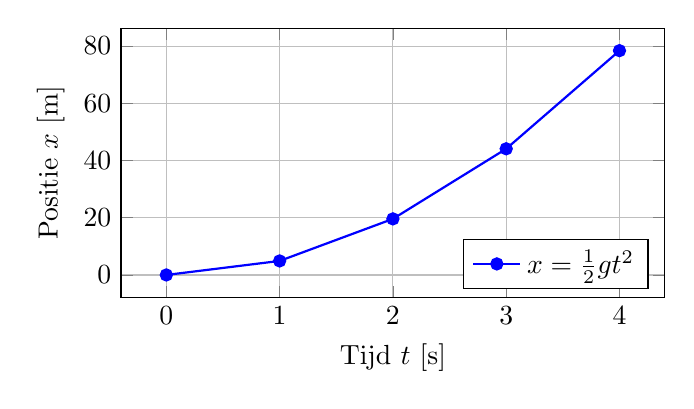
\begin{tikzpicture}
\begin{axis}[
    width=0.7\linewidth,
    height=5cm,
    xlabel={Tijd $t$ [s]},
    ylabel={Positie $x$ [m]},
    grid=major,
    legend pos=south east
]
\addplot[mark=*, blue, thick] coordinates {
    (0,0) (1,4.9) (2,19.6) (3,44.1) (4,78.4)
};
\addlegendentry{$x = \frac{1}{2}gt^2$}
\end{axis}
\end{tikzpicture}
\end{center}

\subsection{Simpele TikZ Figuur}
\begin{center}
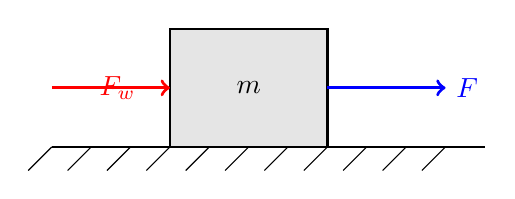
\begin{tikzpicture}
% Blok
\draw[thick, fill=gray!20] (0,0) rectangle (2,1.5);
\node at (1, 0.75) {$m$};
% Kracht pijlen
\draw[->, very thick, blue] (2,0.75) -- (3.5,0.75) node[right] {$F$};
\draw[->, very thick, red] (-1.5,0.75) -- (0,0.75) node[left, xshift=-0.3cm] {$F_w$};
% Grond
\draw[thick] (-1.5,0) -- (4,0);
\foreach \x in {-1.5,-1,...,3.5}
    \draw (\x,0) -- (\x-0.3,-0.3);
\end{tikzpicture}
\end{center}

%=============================================================================
\section{Figuren}
%=============================================================================

\subsection{Standaard Figuur}
\begin{verbatim}
\begin{figure}[H]
    \centering
    \includegraphics[width=0.6\linewidth]{image.png}
    \caption{Beschrijving van de figuur}
    \label{fig:voorbeeld}
\end{figure}
\end{verbatim}

\subsection{Snelle Macro's (school-macros)}
\begin{verbatim}
\fig[0.6\linewidth]{pad/naar/afbeelding.png}{Caption}{fig:label}
\img{afbeelding.png}{Caption}
\end{verbatim}

%=============================================================================
\section{Speciale Boxes (school-macros)}
%=============================================================================

\subsection{Conceptbox — Definities}
\begin{conceptbox}[title=Wet van Newton]
\textbf{Tweede wet}: $\vec{F} = m\vec{a}$

De resultante kracht op een lichaam is gelijk aan de massa maal de versnelling.
\end{conceptbox}

\begin{conceptbox}
Zonder titel — voor korte definities of opmerkingen.
\end{conceptbox}

\subsection{Warningbox — Waarschuwingen}
\begin{warningbox}[title=Let Op!]
Vergeet niet de eenheden om te rekenen naar SI!
\end{warningbox}

\begin{warningbox}
Veelgemaakte fout: $v^2$ vergeten in kinetische energie formule.
\end{warningbox}

\subsection{Oefenblok — Oefeningen}
\begin{oefenblok}[title=Voorbeeld: Vrije Val]
Een voorwerp valt van 20 m hoogte. Bereken de snelheid bij impact.

\textbf{Gegeven:} $h = 20$ m, $g = 9.81$ m/s²

\textbf{Oplossing:}
\[ v = \sqrt{2gh} = \sqrt{2 \cdot 9.81 \cdot 20} = 19.8 \text{ m/s} \]
\end{oefenblok}

\subsection{Examenbox — Examtips}
\begin{examenbox}
Controleer altijd je eenheden! Zet alles om naar SI voordat je rekent.
\end{examenbox}

%=============================================================================
\section{Formule Macro (\textbackslash frm)}
%=============================================================================

De \verb|\frm| macro maakt een formule-box én voegt deze automatisch toe aan het formularium:

\frm{Kinetische Energie}{E_k = \frac{1}{2}mv^2}{$m$ = massa [kg], $v$ = snelheid [m/s]}

\frm{Potentiële Energie}{E_p = mgh}{$m$ = massa [kg], $g$ = 9.81 m/$s^2$, $h$ = hoogte [m]}

\frm{Wet van Ohm}{U = IR}{$U$ = spanning [V], $I$ = stroom [A], $R$ = weerstand [$\Omega$]}

%=============================================================================
\section{Symbool Registratie (\textbackslash sym)}
%=============================================================================

Bij eerste gebruik toont \verb|\sym| een box met uitleg. Daarna alleen het symbool:

\sym{v}{Snelheid}{m/s}
\sym{a}{Versnelling}{m/$s^2$}
\sym{F}{Kracht}{N}
\sym{omega}{Hoeksnelheid}{rad/s}

Later in de tekst: de snelheid $v = 10$ m/s met versnelling $a = 2$ m/$s^2$.

Tweede keer \verb|\sym{v}{...}{...}| geeft alleen: \sym{v}{Snelheid}{m/s}

%=============================================================================
\section{Wiskunde Shortcuts (school-macros)}
%=============================================================================

\subsection{Afgeleiden}
\begin{tabular}{ll}
\verb|\dd{y}{x}| & $\dd{y}{x}$ (gewone afgeleide) \\
\verb|\ddn{y}{x}{2}| & $\ddn{y}{x}{2}$ (tweede afgeleide) \\
\verb|\pd{f}{x}| & $\pd{f}{x}$ (partiële afgeleide) \\
\verb|\pdn{f}{x}{2}| & $\pdn{f}{x}{2}$ (tweede partiële) \\
\end{tabular}

\subsection{Differentialen}
$\int x^2 \, \dx$ \quad $\int v \, \dt$ \quad $\int f \, \dy$

\subsection{Vectoren}
\begin{tabular}{ll}
\verb|\vec{F}| & $\vec{F}$ (vector) \\
\verb|\uvec{n}| & $\uvec{n}$ (eenheidsvector) \\
\verb|\mat{A}| & $\mat{A}$ (matrix) \\
\end{tabular}

Voorbeeld: $\vec{F} = m\vec{a}$

\subsection{Verzamelingen}
$\NN$ (natuurlijk), $\ZZ$ (geheel), $\QQ$ (rationaal), $\RR$ (reëel), $\CC$ (complex)

\subsection{Auto-scaling Haakjes}
\begin{tabular}{ll}
\verb|\abs{x}| & $\abs{\frac{a}{b}}$ \\
\verb|\norm{v}| & $\norm{\frac{a}{b}}$ \\
\verb|\paren{...}| & $\paren{\frac{a}{b}}$ \\
\verb|\bracket{...}| & $\bracket{\frac{a}{b}}$ \\
\verb|\avg{x}| & $\avg{x}$ (gemiddelde) \\
\end{tabular}

%=============================================================================
\section{Referenties}
%=============================================================================

Labels en verwijzingen:
\begin{verbatim}
\begin{equation}\label{eq:newton}
  F = ma
\end{equation}
Zie \eqnref{eq:newton} voor de formule.
\end{verbatim}

\begin{equation}\label{eq:newton}
F = ma
\end{equation}

Verwijzing: zie \eqnref{eq:newton}.

Beschikbare commando's:
\begin{itemize}
\item \verb|\eqnref{label}| / \verb|\Eqnref{label}| — vergelijking
\item \verb|\figref{label}| / \verb|\Figref{label}| — figuur
\item \verb|\tabref{label}| / \verb|\Tabref{label}| — tabel
\item \verb|\secref{label}| / \verb|\Secref{label}| — sectie
\end{itemize}

%=============================================================================
\section{Layout Hulpmiddelen}
%=============================================================================

\subsection{Minipage — Naast Elkaar}
\begin{minipage}{0.48\textwidth}
\textbf{Linker kolom}

Tekst of formules hier.
\[ E = mc^2 \]
\end{minipage}%
\hfill
\begin{minipage}{0.48\textwidth}
\textbf{Rechter kolom}

Meer tekst of een figuur.
\[ F = ma \]
\end{minipage}

\subsection{Meerdere Kolommen}
\begin{multicols}{2}
Tekst in twee kolommen. Handig voor compacte lijsten of veel kleine formules.

De tekst vloeit automatisch.

\columnbreak

Tweede kolom. Gebruik \verb|\columnbreak| voor handmatige overgang.
\end{multicols}

%=============================================================================
\section{Handige Commando's}
%=============================================================================

\subsection{TODO Markers}
\TODO{Nog toevoegen}
\FIXME{Controleer dit}
\NOTE{Onthoud voor examen}

\subsection{Graden}
$45\degree$, $90\degree$, $180\degree$ met \verb|\degree|

\subsection{Chemische Formules}
Met \verb|mhchem| package (automatisch geladen):

\verb|\ce{H2O}| geeft \ce{H2O}

\verb|\ce{2H2 + O2 -> 2H2O}| geeft \ce{2H2 + O2 -> 2H2O}

%=============================================================================
\section{Tips voor Samenvattingen}
%=============================================================================

\begin{enumerate}
\item \textbf{Gebruik \texttt{school-macros}} — consistente opmaak
\item \textbf{Compileer 2×} — voor formularium en symbolenlijst
\item \textbf{Gebruik \texttt{\textbackslash frm}} — voor alle belangrijke formules
\item \textbf{Gebruik \texttt{\textbackslash sym}} — bij eerste vermelding van symbolen
\item \textbf{Gebruik boxes} — \texttt{conceptbox} voor definities, \texttt{warningbox} voor aandachtspunten
\item \textbf{Label alles} — maakt verwijzingen makkelijk
\end{enumerate}

\subsection{Structuur Template}
\begin{verbatim}
\documentclass[a4paper,11pt]{article}
\usepackage{school-macros}

\title{Samenvatting Vak}
\author{Naam}
\date{\today}

\begin{document}
\maketitle
\tableofcontents
\newpage

\section{Onderwerp 1}
\begin{conceptbox}[title=Belangrijke Definitie]
Uitleg hier...
\end{conceptbox}

\frm{Formule Naam}{F = ma}{uitleg variabelen}

\section{Onderwerp 2}
% etc.

\newpage
\printsymbols
\printformularium
\end{document}
\end{verbatim}

%=============================================================================
\appendix
\section*{Symbolenlijst}
\printsymbols

\section*{Formularium}
\printformularium

\end{document}
